\chapter{METHODOLOGY}

This chapter presents the architecture and implementation methods used to build the \textit{\textbf{Smart Boarding House Management System}}.

\section{Tools and Techniques}
Choosing the right tools is very important to build a reliable rental management platform. This section explains the technologies selected for the backend, frontend, supporting services, and system deployment, and the reasons for choosing them instead of other options.

\subsection{Backend Services}
For the backend, \textbf{NestJS} is chosen instead of simple frameworks like \textbf{Express}. \textbf{NestJS} provides a modular structure, dependency injection, and decorators, which makes it easy to organize the codebase. This organization is very helpful for implementing \textbf{Clean Architecture} and keeping the code neat as the system grows. \textbf{PostgreSQL} is used as the primary database because rental data like contracts and invoices must be secure and consistent. To connect the backend with \textbf{PostgreSQL}, \textbf{Prisma ORM} is used because it offers type-safe queries and makes database migrations easy. While \textbf{MongoDB} schemas are present in the codebase for potential logging development, the current active implementation relies entirely on \textbf{PostgreSQL} for data consistency.

\subsection{Frontend Portal}
For the frontend, \textbf{Next.js 14 App Router} is used instead of a standard \textbf{React} single-page application. \textbf{Next.js} offers server-side rendering, which is useful for the public landing page to load faster and have better search engine optimization. It also has a clean routing system that helps separate public pages, landlord admin pages, and the tenant portal. To manage the global application state, \textbf{Zustand} is chosen instead of \textbf{Redux}. \textbf{Zustand} is much lighter, has less boilerplate code, and is easier to learn, while still providing great performance for storing user sessions and UI states. For API requests, \textbf{Axios} is used with custom interceptors to automatically attach landlord identification headers and authorization tokens to every request.

\subsection{Supporting Services and Integrations}
To add special features to the platform, several supporting libraries and services are integrated. \textbf{Socket.IO} is used instead of constant HTTP polling to send notifications. This allows landlords to receive instant alerts when a tenant reports an incident or sends a room request. To store room images, \textbf{Cloudinary} is chosen instead of saving files locally on the server, which helps save disk space and automatically optimizes images for faster loading. For \textbf{AI} features, the \textbf{Google Generative AI} library with the \textbf{Gemini} model is used because it is very fast, accurate, and cost-effective for generating landlord notices and chatting with tenants. Finally, the \textbf{VietQR} image API is used to generate payment QR codes and insert them into invoice \textbf{PDF} files, allowing tenants to pay easily using their banking apps.

\subsection{Infrastructure and Deployment}
For deployment and production hosting, the system uses a serverless cloud infrastructure. The database is hosted on \textbf{Neon}, which provides a serverless \textbf{PostgreSQL} database. This allows the system to store rental data securely with high availability. The \textbf{NestJS} backend is deployed as a Web Service on \textbf{Render}. \textbf{Render} automatically builds the \textbf{NestJS} application from the backend directory and connects it to the \textbf{Neon} database. The \textbf{Next.js} frontend is deployed on \textbf{Vercel} because \textbf{Vercel} is optimized for \textbf{Next.js} applications, offering fast loading speeds. The frontend communicates with the backend on \textbf{Render} using environment variables. Both \textbf{Render} and \textbf{Vercel} are connected to the \textbf{GitHub} repository. This setup enables automatic \textbf{CI/CD} deployment, meaning any new code changes pushed to the repository are automatically built and deployed to the production environment.



\section{System Architecture}
This section describes how the different parts of the Smart Boarding House Management System are organized and connect with each other. The system is designed using a clean, layered structure to separate the user interface, business logic, and database operations.

\subsection{Overall System Structure}
The system follows a \textbf{client-server} architecture. The frontend is built with \textbf{Next.js} and acts as the client side. The backend is built with \textbf{NestJS} and acts as the server side. As shown in Figure \ref{fig:system_architecture}, the client and the server communicate using HTTP \textbf{REST APIs} for standard data requests and \textbf{Socket.IO} for real-time notifications. The backend server connects directly to the \textbf{PostgreSQL} database to read and store information. It also communicates with external services like \textbf{Cloudinary} to upload images, \textbf{Google Gemini} to run \textbf{AI} features, and the \textbf{VietQR API} to get payment codes.

\begin{figure}[H]
    \centering
    
\includegraphics[width=1.0\textwidth]{SystemArchitecture.png}
    \caption{Overall System Architecture}
    \label{fig:system_architecture}
\end{figure}

\subsection{Layered Design}
To make the codebase easy to maintain, the \textbf{backend} and \textbf{frontend} are organized into three distinct layers: the \textbf{presentation layer}, the \textbf{application layer}, and the \textbf{infrastructure layer}.

The \textbf{presentation layer} is the top layer. In the \textbf{backend}, it contains HTTP controllers and data transfer objects to receive requests and send responses. In the \textbf{frontend}, it contains the visual pages and interactive components. The \textbf{presentation layer} does not process business rules; it only passes data to the next layer.

The \textbf{application layer} contains the core business logic of the system. For example, when a landlord creates a contract, the \textbf{application layer} checks if the room is vacant and updates the room status. It contains modules for authentication, room management, contract lifecycles, and invoice creation. This layer is completely independent of the database details or framework configurations.

The \textbf{infrastructure layer} is the bottom layer. It handles communication with external systems. In the \textbf{backend}, it includes database services to execute \textbf{PostgreSQL} queries using \textbf{Prisma}, and call external APIs like \textbf{Cloudinary} and \textbf{Google Generative AI}. This layered design ensures that changes in one part of the system, like upgrading the database, do not affect the rest of the application.


\section{Database Design}
The database is a very important part of the platform because it stores all information about rooms, tenants, contracts, and invoices. \textbf{PostgreSQL} is used as the database and \textbf{Prisma ORM} connects the backend server to it. This section explains the database structure, the relationships between different tables, and how the data is organized.

\subsection{Entity-Relationship Diagram}
To understand how the data is structured, an \textbf{Entity-Relationship Diagram (ERD)} is created. As shown in Figure \ref{fig:erd_diagram}, the database has eight main tables that represent the core parts of the boarding house system. These tables are \textbf{User}, \textbf{Landlord}, \textbf{Room}, \textbf{Contract}, \textbf{Invoice}, \textbf{RentRequest}, \textbf{Incident}, and \textbf{Violation}.

\begin{figure}[H]
    \centering
    
\includegraphics[width=1.0\textwidth]{erd.png}
    \caption{Database Entity-Relationship Diagram}
    \label{fig:erd_diagram}
\end{figure}

\subsection{Core Database Tables}
The \textbf{User} table stores information about all accounts in the system. Each user has an email, password, name, phone, status, and role (which can be \textbf{Admin}, \textbf{Landlord}, or \textbf{Tenant}). If the user is a tenant, they can also have a \textbf{landlordId} to connect them to a specific landlord.

The \textbf{Landlord} table stores the business profile of property owners. It contains details like the landlord's name, phone, address, and bank account information (bank name, account name, and account number). This bank information is used to generate \textbf{VietQR} codes on invoice \textbf{PDF}s automatically.

The \textbf{Room} table contains information about the rental rooms. Each room has a room number, floor, description, rental price, status (which can be \textbf{Vacant}, \textbf{Occupied}, or \textbf{Maintenance}), and a list of image URLs hosted on \textbf{Cloudinary}. Every room is connected to a specific landlord.

The \textbf{Contract} table represents the lease agreement. It connects a tenant user and a room together. It stores the start date, end date, deposit amount, monthly rental price, electricity price, water price, and status (which can be \textbf{Pending}, \textbf{Active}, \textbf{Expired}, or \textbf{Terminated}).

The \textbf{Invoice} table stores monthly billing records. It links to a specific contract and stores the total amount, electric cost, water cost, other costs, due date, payment date, and status (which can be \textbf{Unpaid}, \textbf{Paid}, \textbf{Overdue}, or \textbf{Cancelled}).

The \textbf{RentRequest} table stores requests from public visitors who want to ask about rooms. The \textbf{Incident} table stores repair and maintenance requests submitted by tenants. The \textbf{Violation} table stores rules violations recorded by landlords.

\subsection{Multi-Tenant Data Privacy}
To keep the data of each landlord private, the system uses a multi-tenant design. Most tables in the database, including \textbf{Room}, \textbf{Contract}, \textbf{Invoice}, \textbf{RentRequest}, \textbf{Incident}, and \textbf{Violation}, contain a \textbf{landlordId} field. When a landlord logs in, the \textbf{backend} server automatically filters all queries using their \textbf{landlordId}. This ensures that a landlord can only see their own rooms, contracts, and invoices, and cannot access data belonging to other landlords.


\section{Authentication and Authorization}
Security is a critical part of the Smart Boarding House Management System. The platform must ensure that only registered users can access private pages, and that landlords can only see their own rental data. To implement this, the backend uses token-based authentication and role-based access control.

\subsection{User Authentication with JWT}
The system uses JSON Web Tokens (JWT) to authenticate users. When a user logs in by entering their email and password, the authentication service validates their credentials. If the information is correct, the server generates a signed JWT token and returns it to the client. This token contains a payload with the user's identification code, email address, role, and landlord identification code. For every subsequent request, the client must send this token in the HTTP Authorization header as a Bearer token. To validate these tokens, the backend uses a NestJS Passport strategy. This strategy extracts the token, verifies its signature using a secret key, and automatically attaches the decoded user data to the request object as the authenticated user. The structure of this JWT token payload is described in Table \ref{tab:jwt_payload}.

\begin{table}[H]
    \centering
    \renewcommand{\arraystretch}{1.2}
    \begin{tabular}{|l|l|p{8cm}|}
        \hline
        \textbf{Claim Key} & \textbf{Data Type} & \textbf{Purpose and Description} \\
        \hline
        sub & String (UUID) & The unique identifier of the authenticated User. \\
        \hline
        email & String & The email address used to identify the user account. \\
        \hline
        role & Enum & The system role of the user (e.g., ADMIN, LANDLORD, or TENANT). \\
        \hline
        landlordId & String (UUID) & The landlord identifier used to filter data access for multi-tenancy. \\
        \hline
    \end{tabular}
    \caption{Structure of the JSON Web Token (JWT) Payload}
    \label{tab:jwt_payload}
\end{table}

\subsection{API Protection with Auth Guards}
To protect individual API endpoints, the backend implements custom NestJS guards. The primary guard is the JWT Auth Guard, which intercepts incoming requests to protected routes. If the request does not contain a valid token, the guard blocks the request and throws an unauthorized exception. For routes that require specific roles, the system combines the JWT Auth Guard with a Roles Guard. The Roles Guard uses a custom Roles decorator and the NestJS Reflector to read the roles allowed for a route. It checks the role of the logged-in user inside the request object and compares it with the required roles. For example, if a route is decorated for landlords only, a tenant attempting to access it will be blocked and receive a forbidden exception. The flowchart in Figure \ref{fig:auth_guard_flowchart} shows how requests are processed through these guards.

\begin{figure}[H]
    \centering
    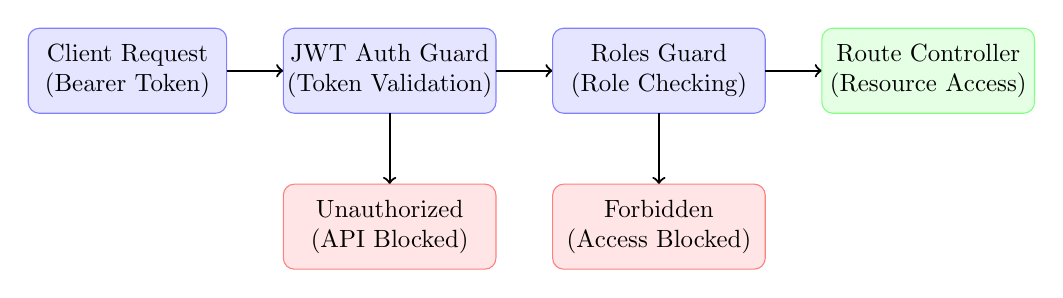
\begin{tikzpicture}[scale=0.9, every node/.style={transform shape}]
        \draw[fill=blue!10, draw=blue!50, rounded corners] (0,0) rectangle (2.8,1.2) node[pos=.5, align=center] {Client Request \\ (Bearer Token)};
        \draw[->, thick] (2.8,0.6) -- (3.6,0.6);
        \draw[fill=blue!10, draw=blue!50, rounded corners] (3.6,0) rectangle (6.6,1.2) node[pos=.5, align=center] {JWT Auth Guard \\ (Token Validation)};
        \draw[->, thick] (6.6,0.6) -- (7.4,0.6);
        \draw[fill=blue!10, draw=blue!50, rounded corners] (7.4,0) rectangle (10.4,1.2) node[pos=.5, align=center] {Roles Guard \\ (Role Checking)};
        \draw[->, thick] (10.4,0.6) -- (11.2,0.6);
        \draw[fill=green!10, draw=green!50, rounded corners] (11.2,0) rectangle (14.2,1.2) node[pos=.5, align=center] {Route Controller \\ (Resource Access)};
        
        \draw[->, thick] (5.1,0) -- (5.1,-1);
        \draw[fill=red!10, draw=red!50, rounded corners] (3.6,-2.2) rectangle (6.6,-1) node[pos=.5, align=center] {Unauthorized \\ (API Blocked)};
        
        \draw[->, thick] (8.9,0) -- (8.9,-1);
        \draw[fill=red!10, draw=red!50, rounded corners] (7.4,-2.2) rectangle (10.4,-1) node[pos=.5, align=center] {Forbidden \\ (Access Blocked)};
    \end{tikzpicture}
    \caption{Authentication and Authorization Guard Flowchart}
    \label{fig:auth_guard_flowchart}
\end{figure}

\subsection{Multi-Tenant Authorization Filter}
Apart from roles, the system enforces multi-tenant authorization using the landlord identification code. Because multiple landlords share the same database, the \textbf{backend} must prevent cross-tenant access. During authentication, the landlord's unique identification code is stored inside the \textbf{JWT} token. When a landlord requests room listings, contracts, or invoice records, the corresponding backend service reads this \textbf{landlordId} code directly from the request user object. The database query then filters the results based on this code. This technique guarantees that landlords can never view or modify the records of other property owners, even if they try to bypass the frontend interface.



\section{Automation and Business Logic}
This section describes the technical implementation of key business processes in the \textbf{backend}. To ensure data consistency and provide a good user experience, the system automates several workflows using database transactions, real-time messaging, and scheduled background tasks. These automated tasks include contract expiration checks, which run daily to return rooms to vacant status when leases end, and startup consistency checks, which automatically fix any room marked occupied that lacks an active contract.

\subsection{Rental Contract Creation}
Creating a new rental contract requires updating multiple records at the same time. As shown in the activity diagram (Figure \ref{fig:activity_create_contract}), when a landlord creates a contract, the system must verify room availability, save the contract details, and update the room status to occupied. To implement this safely, the \textbf{NestJS} backend uses a \textbf{Prisma} database transaction. This transaction guarantees that if any step fails (for example, if the tenant is invalid), the database rolls back to its previous state. This prevents bugs where a contract is created but the room remains vacant, or a room is marked occupied without an active contract.

\begin{figure}[H]
    \centering
    
\includegraphics[width=0.75\textwidth]{activity_create_contract.png}
    \caption{Activity Diagram - Contract Creation Process}
    \label{fig:activity_create_contract}
\end{figure}

\subsection{Invoice Payment and Verification}
The monthly billing cycle is managed through automated invoice generation and a structured payment verification flow. At the beginning of each month, a \textbf{NestJS} cron job runs automatically to create unpaid invoices for all active contracts. As shown in the activity diagram (Figure \ref{fig:activity_invoice_payment_verification}), once an invoice is created, the tenant can view it and scan the generated \textbf{VietQR} code to make a bank transfer. After transferring the money, the tenant marks the invoice as paid in the portal, which immediately changes its status to \textbf{Paid} and records the payment timestamp. The backend simultaneously broadcasts a real-time \textbf{Socket.IO} notification to the landlord's dashboard. The landlord can then manually verify the bank transfer and, if necessary, adjust the invoice status through the administration panel.

\begin{figure}[H]
    \centering
    
\includegraphics[width=0.75\textwidth]{activity_invoice_payment_verification.png}
    \caption{Activity Diagram - Invoice Payment and Verification}
    \label{fig:activity_invoice_payment_verification}
\end{figure}

\subsection{Tenant Incident Handling}
Managing room repairs quickly requires close cooperation between tenants and landlords. As shown in the activity diagram (Figure \ref{fig:activity_tenant_incident_handling}), the process starts when a tenant submits a new incident report with a priority level. The \textbf{backend} saves the incident in the database with a pending status and immediately broadcasts a \textbf{WebSocket} event to the landlord's dashboard using \textbf{Socket.IO}. The landlord reviews the incident, assigns a technician, and updates the status to in-progress. Once the issue is fixed, the landlord marks it as resolved. The system updates the status in the database and sends a real-time message back to the tenant's portal to notify them.

\begin{figure}[H]
    \centering
    
\includegraphics[width=0.75\textwidth]{activity_tenant_incident_handling.png}
    \caption{Activity Diagram - Tenant Incident Handling}
    \label{fig:activity_tenant_incident_handling}
\end{figure}


\section{AI Integration}
The platform integrates advanced artificial intelligence and optical character recognition to automate administrative workflows and improve communication. This section describes how the AI assistant and the OCR utility meter reader are built and how they process data.

\subsection{AI Assistant with Google Gemini}
The \textbf{AI} service is built using the official \textbf{Google Generative AI} library and the \textbf{Gemini 3.1 Flash Lite} model. This model was chosen because it provides fast responses and is highly accurate for text processing. The system implements three distinct assistant modes to help different users, as summarized in Table \ref{tab:ai_modes}.

\begin{table}[H]
    \centering
    \renewcommand{\arraystretch}{1.2}
    \begin{tabular}{|p{3cm}|p{3.5cm}|p{6.5cm}|}
        \hline
        \textbf{Assistant Mode} & \textbf{Database Context Injected} & \textbf{Core Capability} \\
        \hline
        Notice Generator & None (Direct prompt input) & Generates polite, formal boarding house announcements in Vietnamese. \\
        \hline
        RentBot (Public) & Room number, rental price, floor, status, description. & Answers visitor questions about vacant rooms and directs them to register. \\
        \hline
        Tenant Assistant & Contract dates, monthly rent, deposits, unpaid invoices, violations, incidents. & Provides personalized rental Q\&A, checks bills, and explains rules. \\
        \hline
    \end{tabular}
    \caption{Comparison of AI Assistant Modes and Data Contexts}
    \label{tab:ai_modes}
\end{table}

The first mode is notice generation for landlords. Landlords often need to send announcements to all tenants, which can take time to write politely. The landlord can type a simple request in the dashboard, and the \textbf{AI} service automatically generates a formal, polite, and clear announcement in Vietnamese, ready to be sent.

The second mode is the public room consultation chatbot. When visitors browse the landing page, they can chat with an assistant named \textbf{RentBot}. To prevent the \textbf{AI} from making up incorrect information, the \textbf{backend} first queries the \textbf{PostgreSQL} database for actual room numbers, prices, and availability status. The system formats this room list as context and sends it along with the user's question to the \textbf{Gemini} model. This ensures that the assistant only gives accurate answers about vacant rooms and instructs visitors how to apply.

The third mode is the contextual tenant portal assistant. Inside the tenant portal, renters can chat with a personal assistant. When a tenant opens the chat, the \textbf{backend} service queries the database for their specific active contract, invoice history, reported incidents, and open rule violations. It formats this personal data into a detailed system context for the \textbf{Gemini} model. Because the \textbf{AI} has this context, the tenant can ask personalized questions like when their rent is due, how much they owe, or if their reported incident is resolved. The \textbf{AI} answers using the real-time data, providing a personalized self-service experience. The flow of how this personalized prompt is constructed is shown in Figure \ref{fig:ai_prompt_flow}.

\begin{figure}[H]
    \centering
    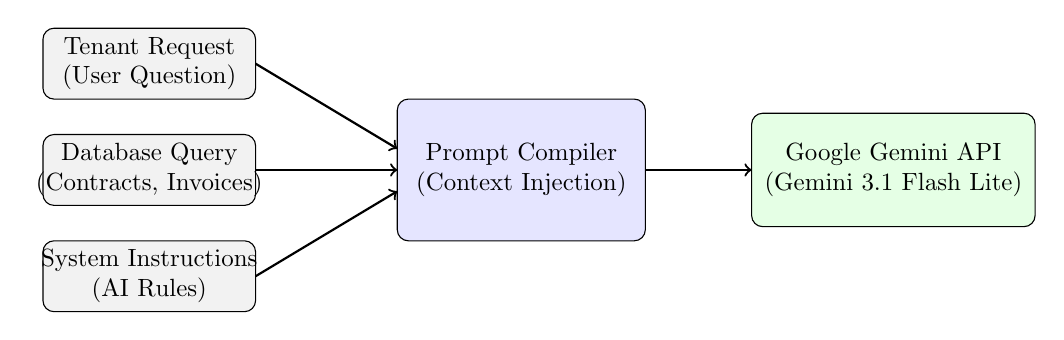
\begin{tikzpicture}[scale=0.9, every node/.style={transform shape}]
        \draw[fill=gray!10, rounded corners] (0,3) rectangle (3,4) node[pos=.5, align=center] {Tenant Request \\ (User Question)};
        \draw[fill=gray!10, rounded corners] (0,1.5) rectangle (3,2.5) node[pos=.5, align=center] {Database Query \\ (Contracts, Invoices)};
        \draw[fill=gray!10, rounded corners] (0,0) rectangle (3,1) node[pos=.5, align=center] {System Instructions \\ (AI Rules)};
        
        \draw[->, thick] (3,3.5) -- (5.0,2.3);
        \draw[->, thick] (3,2) -- (5.0,2);
        \draw[->, thick] (3,0.5) -- (5.0,1.7);
        
        \draw[fill=blue!10, rounded corners] (5.0,1) rectangle (8.5,3) node[pos=.5, align=center] {Prompt Compiler \\ (Context Injection)};
        \draw[->, thick] (8.5,2) -- (10.0,2);
        
        \draw[fill=green!10, rounded corners] (10.0,1.2) rectangle (14.0,2.8) node[pos=.5, align=center] {Google Gemini API \\ (Gemini 3.1 Flash Lite)};
    \end{tikzpicture}
    \caption{Contextual AI Prompt Construction Flowchart}
    \label{fig:ai_prompt_flow}
\end{figure}




